
Nei diagrammi di sequenza viene illustrata la sequenza di operazioni necessarie alla realizzazione degli use case del sistema rispetto agli elementi dell'architettura e alle classi di analisi presenti nel sistema.

Gli use case di HBS possono essere categorizzati, a grandi linee, nelle seguenti categorie:
\begin{itemize}
	\item \emph{transazioni}, per gli use case riguardanti le operazioni che i clienti della banca possono effettuare (incluse le operazioni veloci);

	\item interazioni con il sistema di bidding;

	\item operazioni di gestione del sistema di HBS da parte dei dipendenti della banca.
\end{itemize}

\subsubsection{Transazioni}

Gli use case di tipo \emph{transazionale} seguono uno di due modelli:
\begin{itemize}
	\item modello transazionale semplice;

	\item modello transazionale con conferma tramite OTP.
\end{itemize}

In figura~\ref{fig:sequence:transazione:modello} viene indicato il modello transazionale semplice.

\begin{figure*}[h]
	\centering
	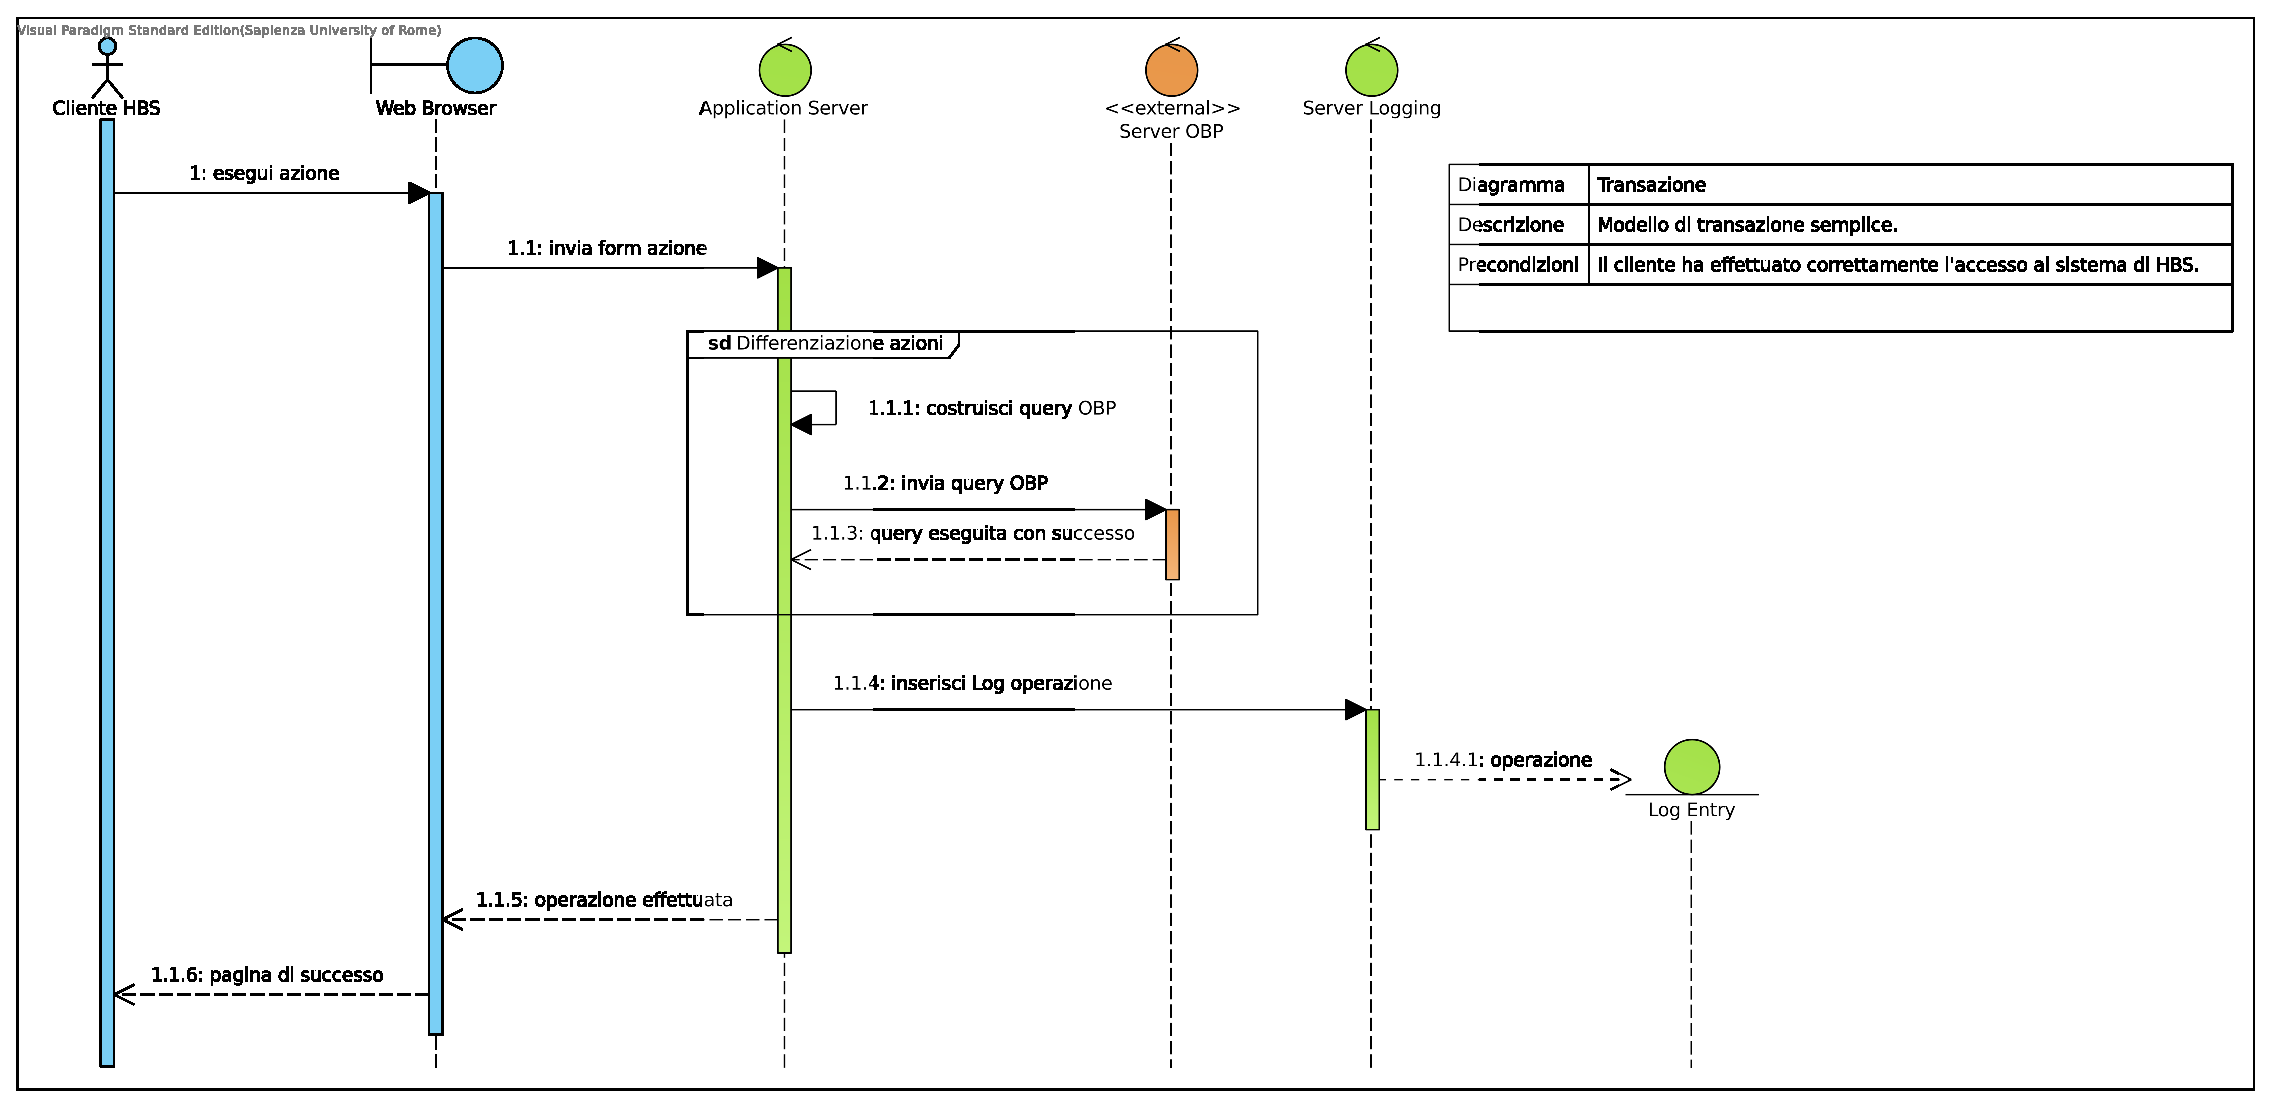
\includegraphics[width=\textheight, angle=90]{Images/sequence/Transazione.eps}
	\caption{Modello di transazione semplice.}
	\label{fig:sequence:transazione:modello}
\end{figure*}

In figura~\ref{fig:sequence:transazione-otp:modello} viene indicato il modello transazionale con conferma tramite OTP.
Use case di questo tipo sono, ad esempio, gli use case riguardanti le operazioni effettuabili da un conto bancario.

\begin{figure*}[h]
	\centering
	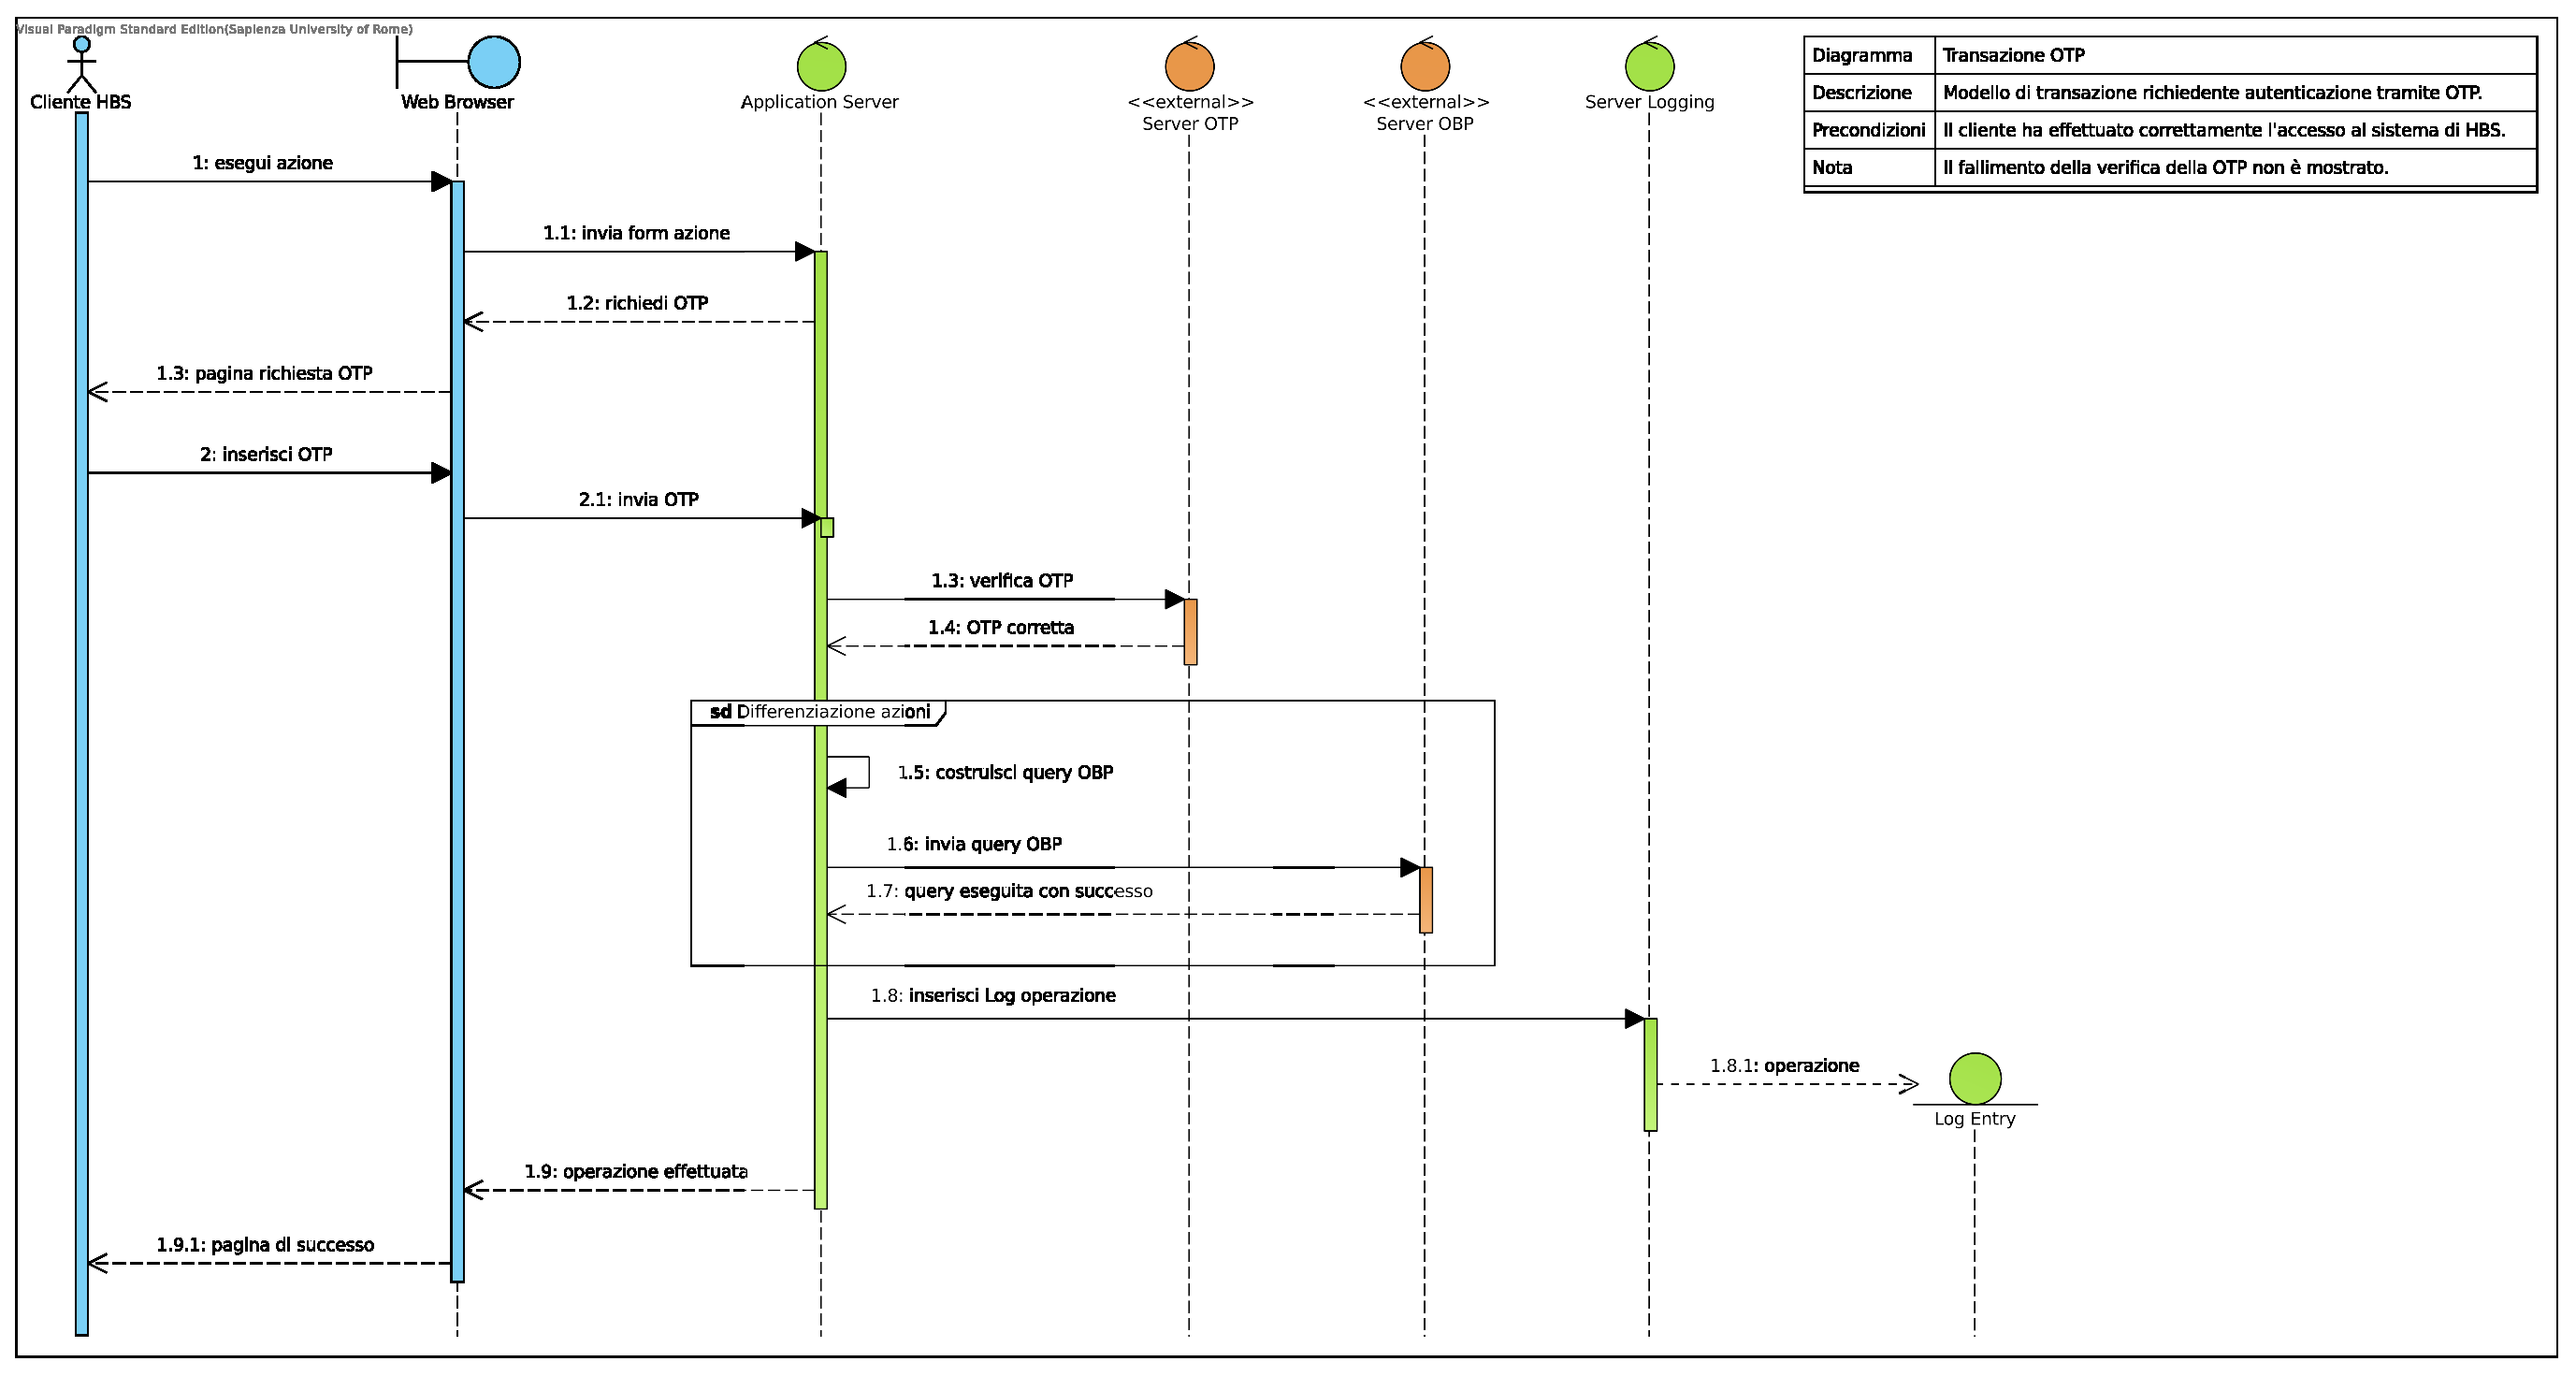
\includegraphics[width=\textheight, angle=90]{Images/sequence/Transazione_OTP.eps}
	\caption{Modello di transazione per la quale è richiesta la conferma tramite OTP.}
	\label{fig:sequence:transazione-otp:modello}
\end{figure*}

\subsubsection{Operazioni}

Le operazioni bancarie effettuabili tramite il sistema di HBS vengono trasmesse da HBS al back-end della banca tramite l'interfaccia di OBP.

L'interfaccia di OBP è una interfaccia RESTful\footnote{L'interfaccia di OBP, in realtà, è in sola lettura. Estendiamo il suo funzionamento anche alla scrittura (inserimento di informazioni nel back-end), poiché l'estensione delle sue funzionalità in questo senso è, almeno logicamente, immediata.}, in cui i dati vengono trasmessi in formato json, e l'autenticazione è gestita tramite protocollo OAuth.

Inserire un'operazione bancaria nel back-end della banca avviene con il seguente messaggio:
\begin{lstlisting}[basicstyle=\ttfamily]
POST /banks/BANK_ID/accounts/ACCOUNT_ID/transactions HTTP/1.1
[header]

{
    "this_account": {
        "id":"ACCOUNT_ID",
        "number": "",
        "kind": "",
        "IBAN": "",
        "swift_bic":"",
        "bank": {
            "national_identifier": "",
            "name": ""
        }
    },
    "other_account": {
        "id":"123213",
        "holder": {
            "name": "DEUTSCHE POST AG, SSC ACC S",
            "is_alias": "true/false"
        },
        "number": "",
        "kind": "",
        "IBAN": "",
        "swift_bic":"",
        "bank": {
            "national_identifier": "",
            "name": ""
        },
    },
    "details": {
        "posted_by_user_id": "user_id",
        "posted_by_ip_address": "ip address",
        "type": "cash",
        "description": "transaction description",
        "posted": "2012-03-07T00:00:00.001Z",
        "completed": "2012-03-07T00:00:00.001Z",
        "value": {
            "currency": "EUR",
            "amount": "-1.45"
        }
    }
}
\end{lstlisting}

Effettuare operazioni veloci (use case \iducDISOPVEL) richiede la creazione di un'operazione ordinaria a partire da un'operazione veloce.
La traduzione da operazione veloce a operazione ordinaria avviene attraverso realizzazioni dell'interfaccia di Traduzione Operazione Veloce.
Ciascun parametro dell'operazione veloce viene tradotto in un parametro dell'operazione ordinaria.
In figura~\ref{fig:sequence:operazione-veloce} viene illustrata la traduzione di un'operazione veloce in un'operazione ordinaria.
Il diagramma di sequenza in figura~\ref{fig:sequence:operazione-veloce} si inserisce nel modello di transazione con conferma tramite OTP illustrato in figura~\ref{fig:sequence:transazione-otp:modello}.

I meccanismi di traduzione possono essere di diverso tipo.
Un meccanismo comune consiste nell'utilizzo

\begin{figure*}[h]
	\centering
	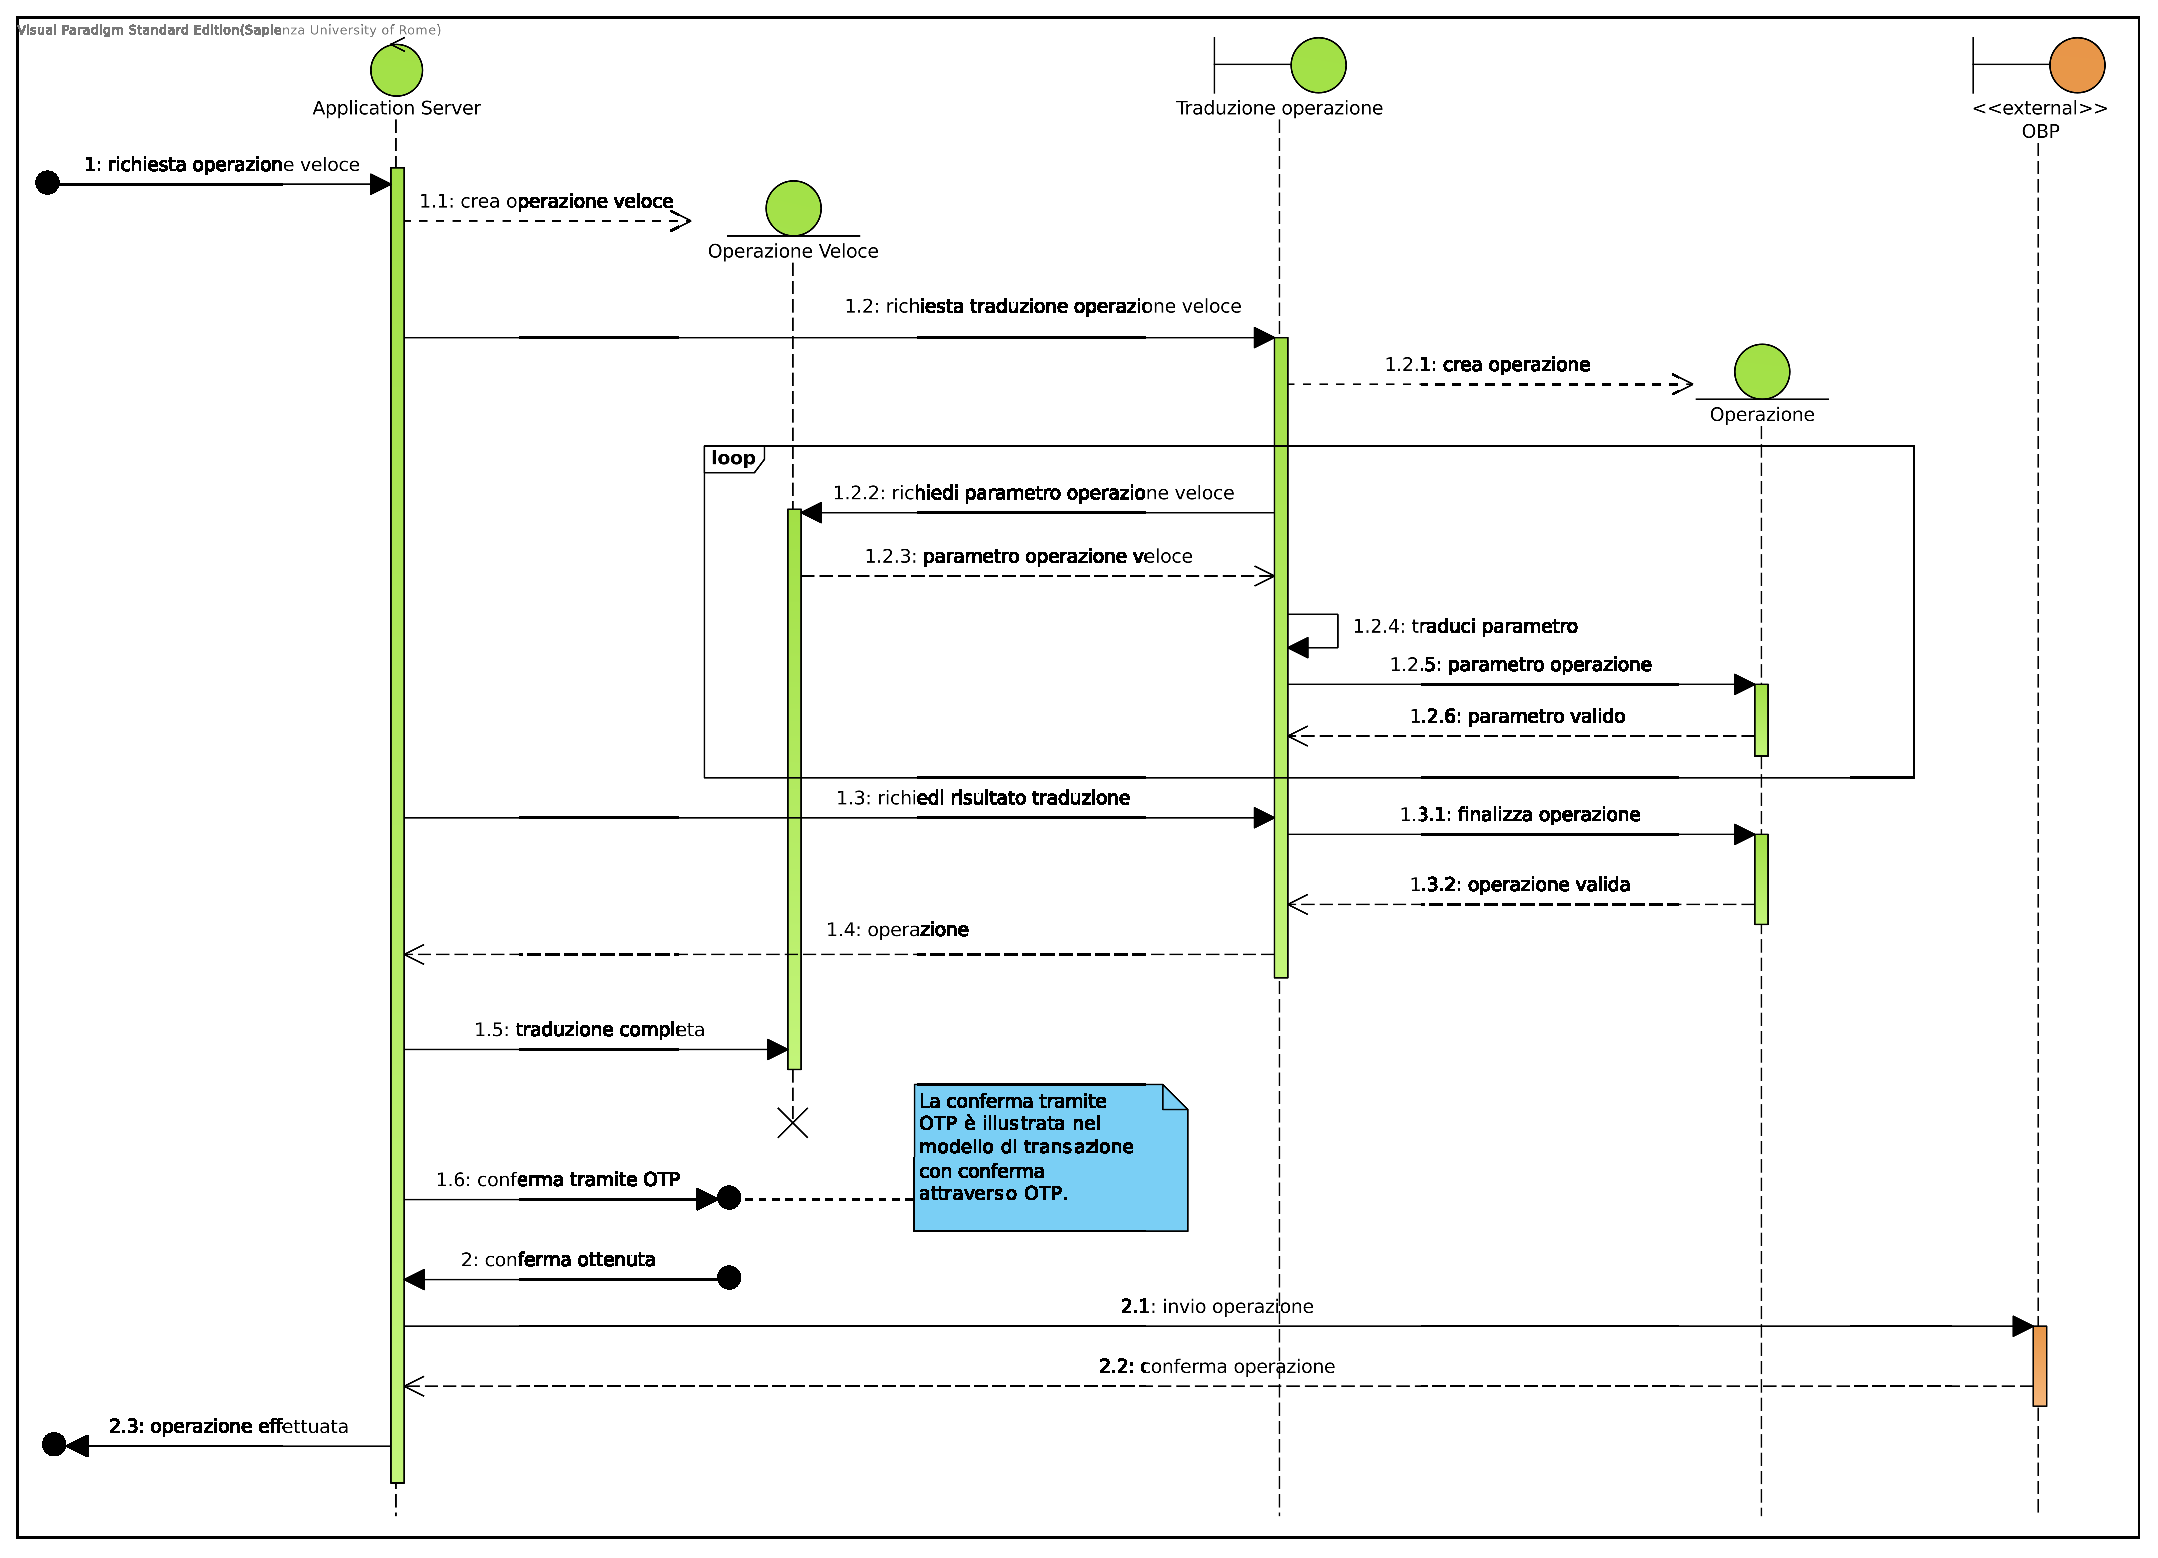
\includegraphics[width=\textheight, angle=90]{Images/sequence/Operazione_Veloce.eps}
	\caption{Traduzione di un'operazione veloce in un'operazione ordinaria.}
	\label{fig:sequence:operazione-veloce}
\end{figure*}

\subsubsection{Dipendenti}
